\section{Introduction}
\label{sec:intro}
Memory accesses are one of the most vital parts of any program. A program is intrinsically made up of loads and stores to the memory. As illustrated in Figure~\ref{fig:cpuvsmemory}, we have witnessed an increasing difference between the performance of processors and memory systems as we move along the Moore's law~\cite{Wulf1995}.  Even with the saturation/demise of the Moore's law~\cite{waldrop2016, MooreMITR}, processing power is expected to grow with the increased reliance on multi-core architectures\cite{Geer}. Since an end-to-end performance of a program heavily depends on both the performance of processor and memory, slower memory becomes a bottleneck and slows down the whole system. {\color{red}This motivates computer architects to explore various ingenious ways to keep memory access latency as short as possible, including sustained efforts towards enhancing the memory hierarchy\cite{Burger}.} Despite these continuous efforts, long-latency memory accesses do occur when there is a miss in the last level cache (LLC). This triggers an access to shared memory, where the processor has to wait for the shared memory to return the requested information. Such waits create stall in the processors. 

%---------------------------
\begin{figure}[t!]
\centering
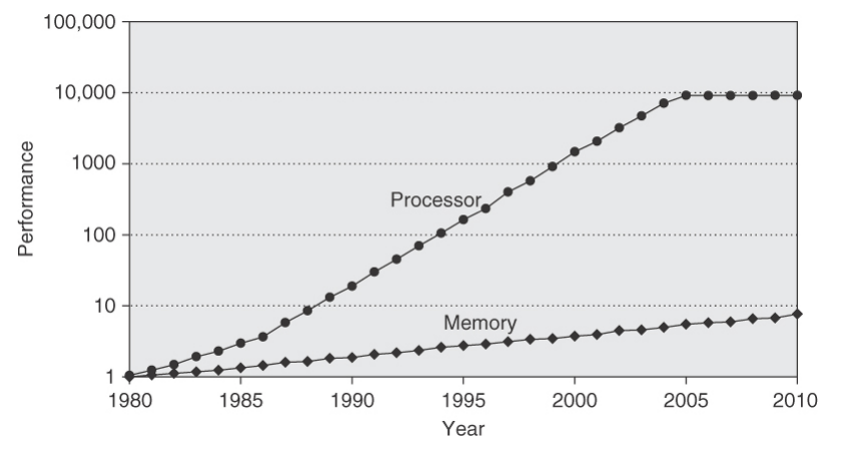
\includegraphics[width=0.7\linewidth]{fig/cpuvsmemory.jpg}
\caption{The gap in performance, measured as the difference in the time 
between processor memory requests (for a single processor or core) and the 
latency of a DRAM access, is plotted over a $30$ year span~\cite{comparchbook}.}
\label{fig:cpuvsmemory}
\end{figure}
%---------------------------
In case of multi-core processor architecture, the problem of stalls gets exacerbated even more as access latency to the 
shared memory increases due to contention among requests issued by different cores. This results in formation of large access request queues waiting to be served  by the slow shared memory. Figure~\ref{fig:multicore_arch}  illustrates a general multi-core 
architecture where $N$ processor cores share a memory consisting of $M$ banks. The access requests from each core is sent to the memory controller first, which then arbitrates and in turn issues (schedules) requests to the memory. Because the memory controller has parallel access to all $M$ banks, a bank queue is used for each individual bank request. These bank queues are 
served every memory clock cycle and the acknowledgement with data (in the case of a 
read) is sent back to the corresponding processor.

In the scenario where multiple cores request access to the memory locations which belong to the same bank, the memory controller puts these request in the respective bank queues. This contention between cores to access from 
the same bank is known as a {\em bank conflict}. In a typical memory system, the bank conflicts lead to the contentious request being served in a sequential manner. Consequently, some of the cores have to wait longer for their request to be fulfilled. As the number of bank conflicts increase, the latency for memory accesses to the bank grows and results into the slow down of the entire system. \\ 
%---------------------------
\begin{figure}[t!]
\centering
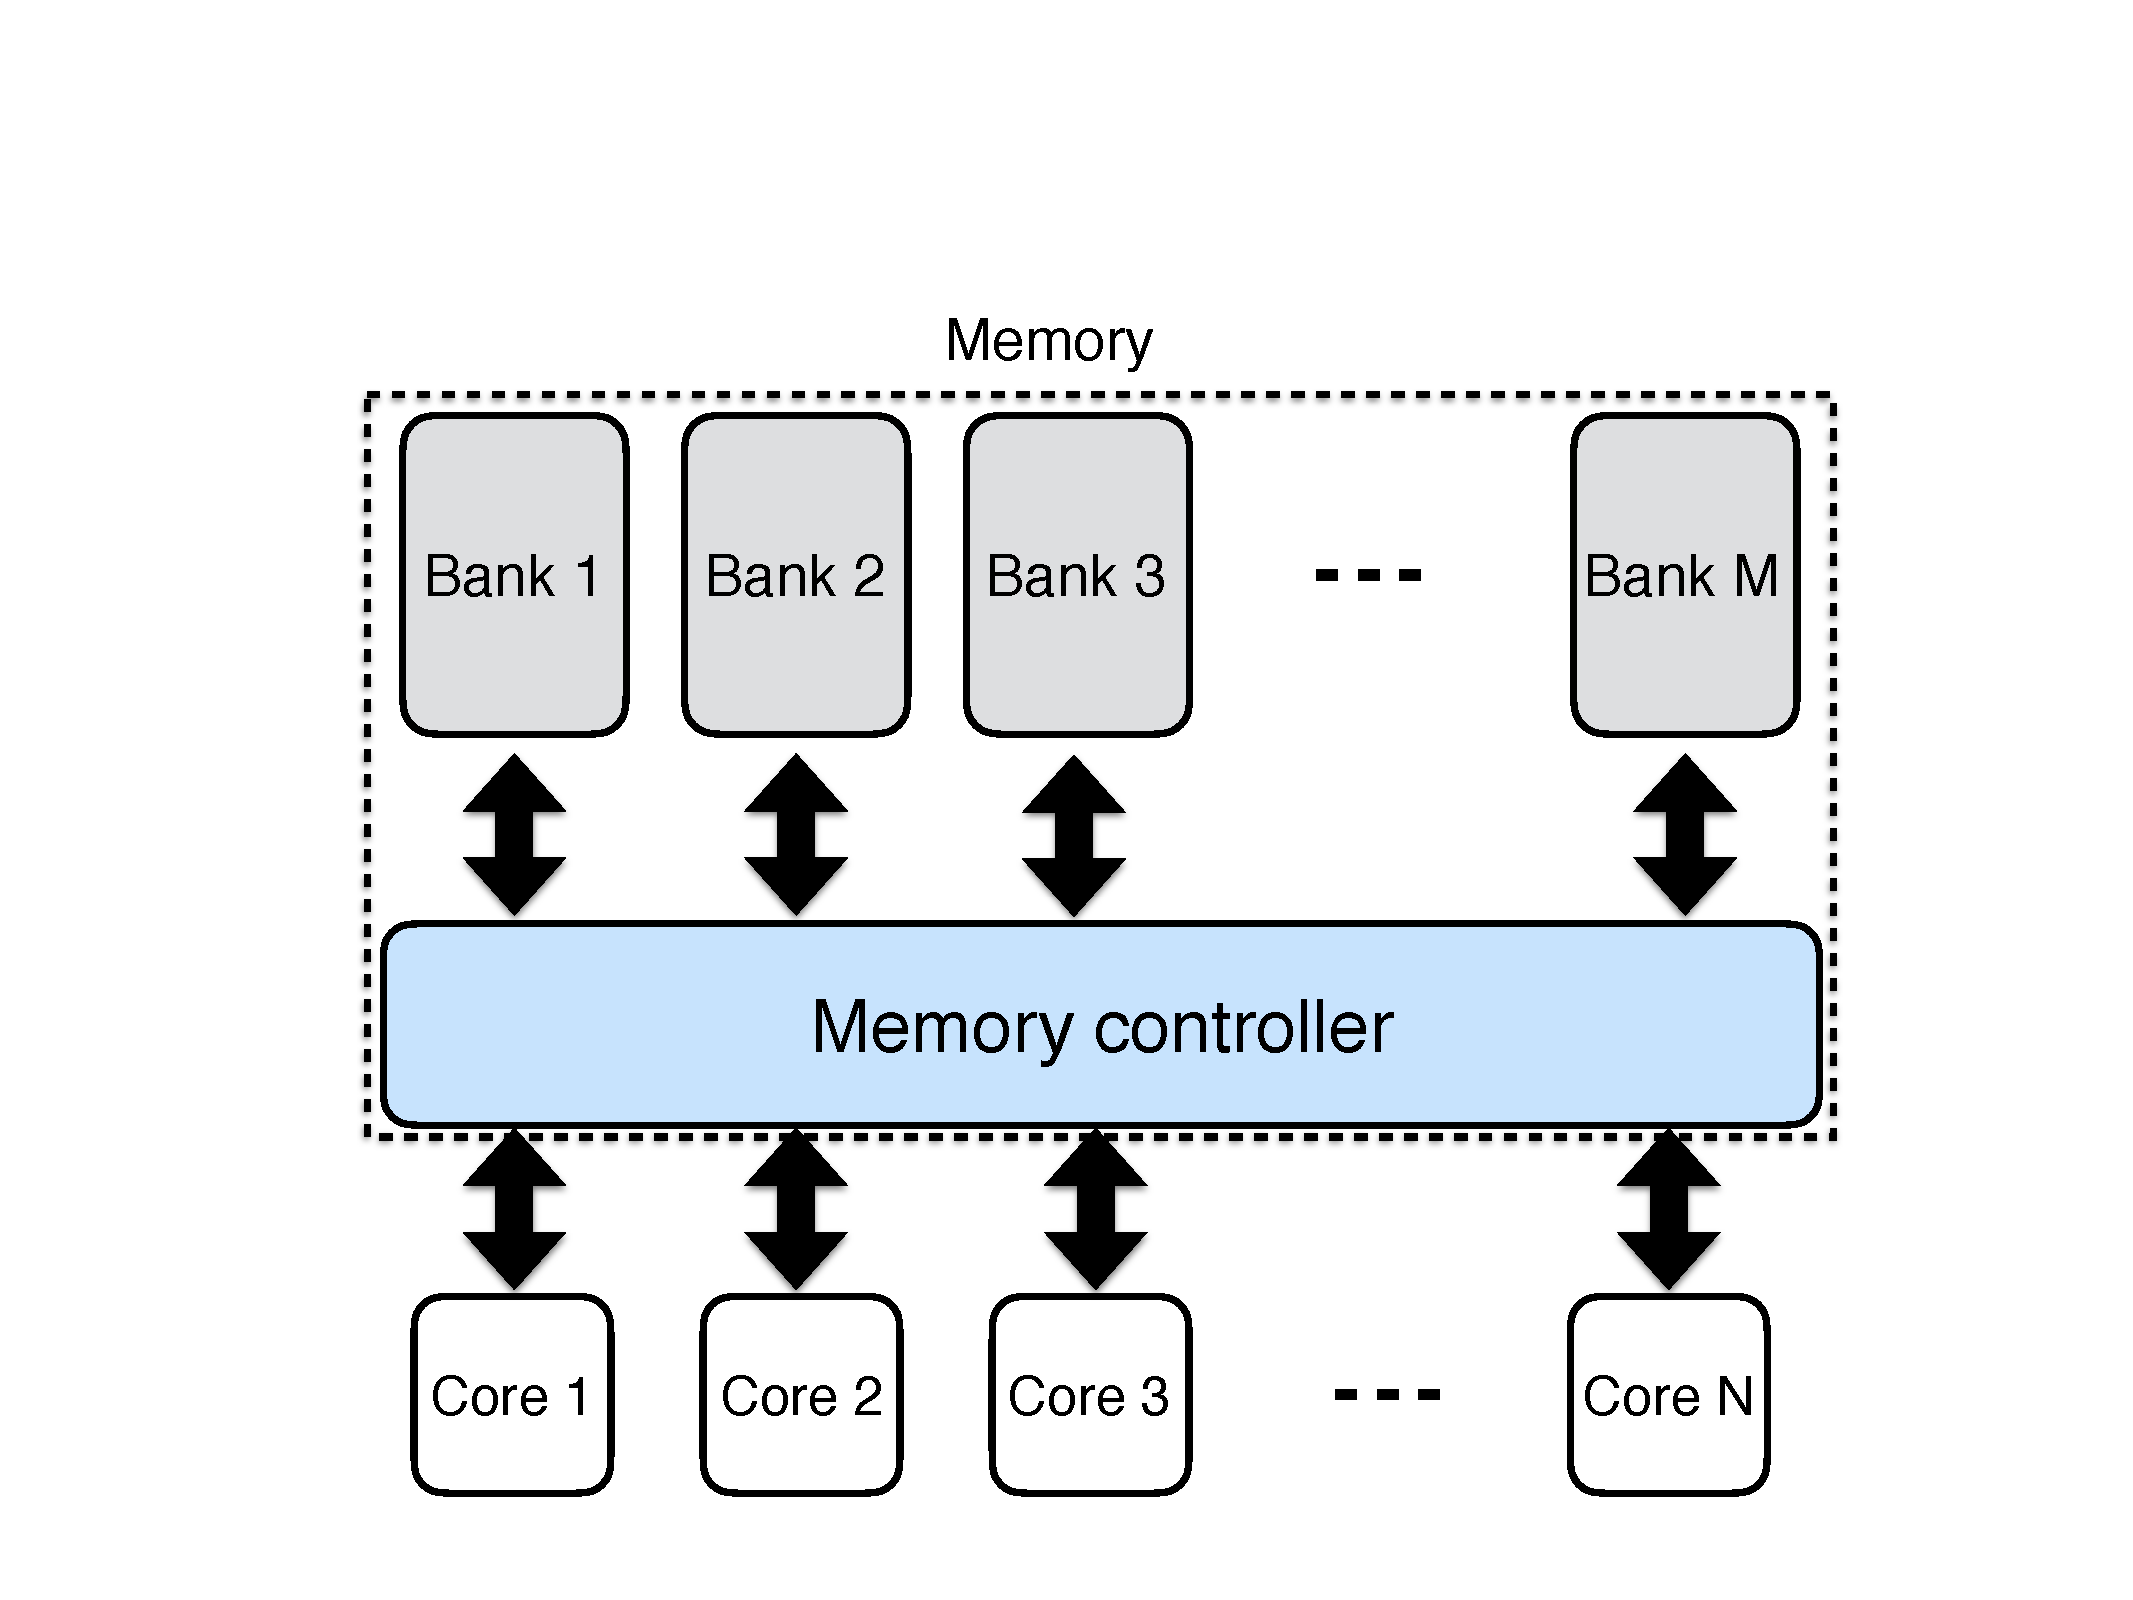
\includegraphics[width=0.6\linewidth]{fig/multicore-sys.pdf}
\caption{General multi-core architecture with a shared memory.}
\label{fig:multicore_arch}
\end{figure}
%---------------------------
In this paper, we aim to address the issue of increased latency due to bank conflicts. The key idea behind our memory design is to distribute the accesses intended for the information stored in a particular bank across multiple banks in the memory. In order to achieve this goal, we rely on coding theoretic techniques to create redundancy across memory banks. That is, we store the information in the memory banks in such a manner that it is possible to recover the information stored on a particular bank by utilizing the information stored in other memory banks. This allows us to simultaneously serve multiple read requests intended for a particular bank, one read request by directly accessing the bank and other requests by querying other banks in the systems. In Figure~\ref{fig:example_xor}, we illustrate this with the help of an example. The setup in Figure~\ref{fig:example_xor} comprises $3$ memory banks where the third bank being redundant as its content is function of the content stored on the first two memory banks. Such redundant banks are also referred to as {\em parity banks}. Assume that the information is arranged in $L$ rows in two first two banks, represented by $[a(1),\ldots, a(L)]$ and $[b(1),\ldots, b(L)]$, respectively. Then the third bank store $L$ rows containing $[a(1) + b(1),\ldots, a(L) + b(L)]$, where $+$ denotes the XOR (modulo $2$ addition) operation. As illustrated in Figure~\ref{fig:example_xor}, this design allows us to simultaneously serve any two read requests (irrespective of their association with first two banks) in a single memory clock cycle. Here, we assume the memory controller to be capable of performing necessary decoding operations, e.g., recovering $a(j)$ from $b(j)$ and $a(j) + b(j)$.

%---------------------------
\begin{figure}[t!]
\centering
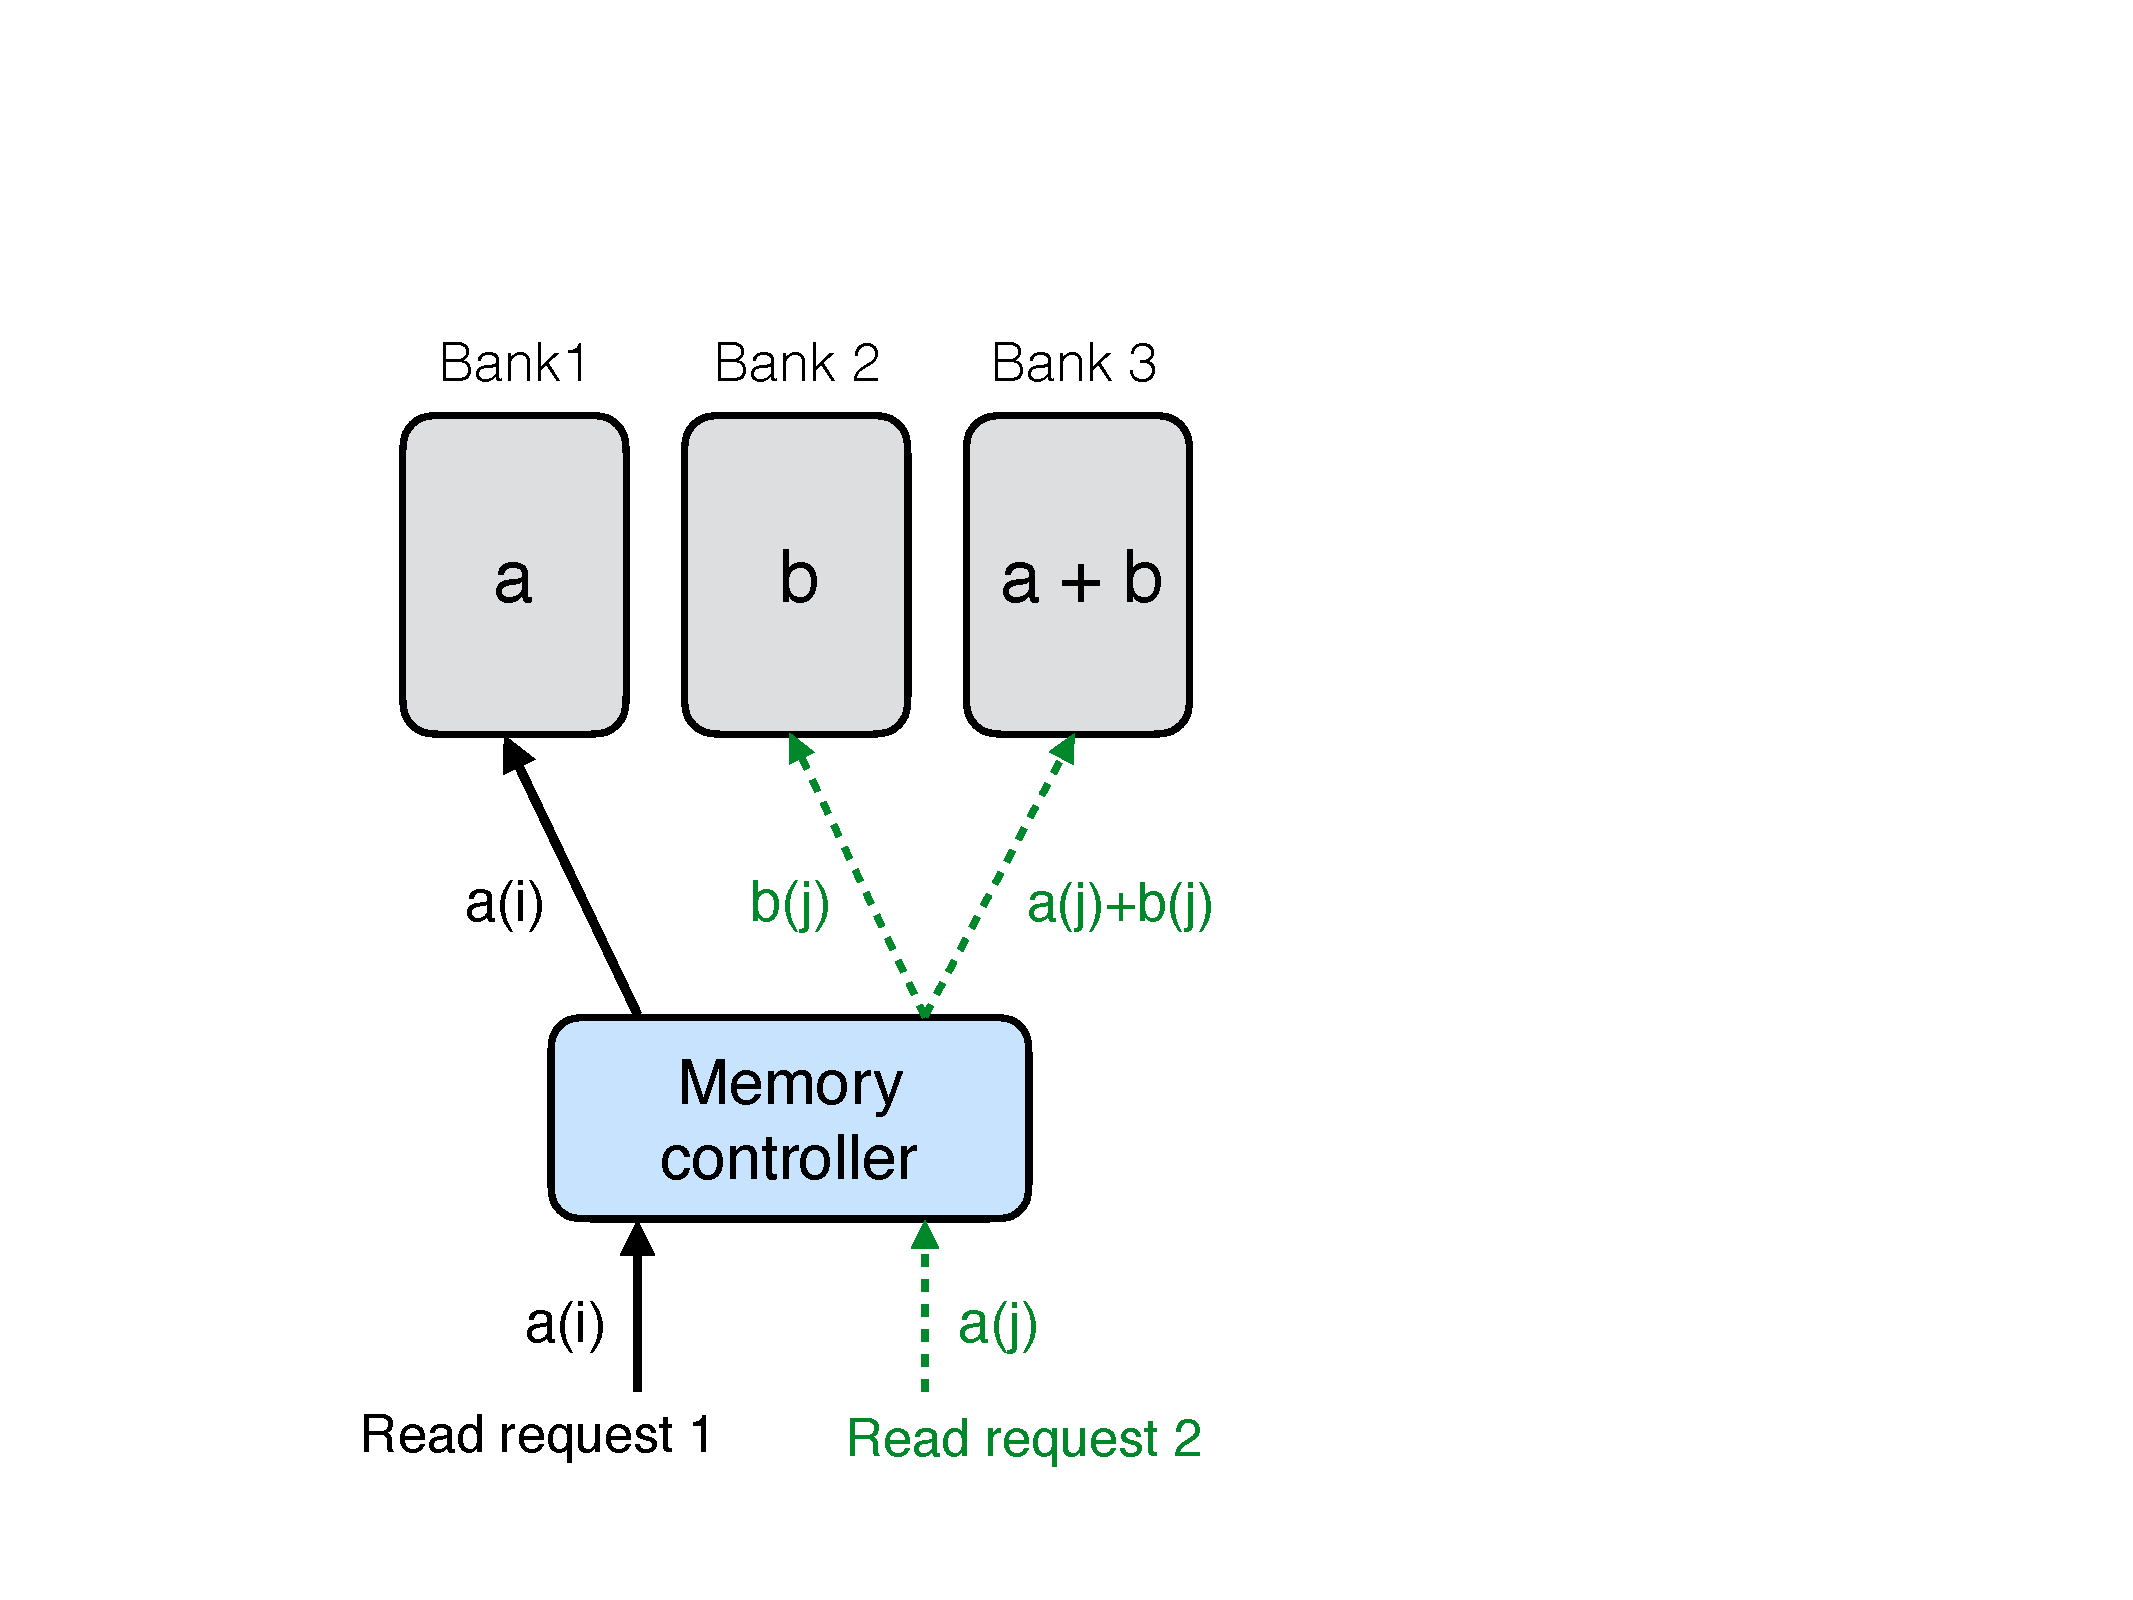
\includegraphics[width=0.395\linewidth]{fig/example-xor.pdf}
\caption{Enabling multiple read accesses to a bank by coding. Given two read requests $\{a(i), a(j)\}$ directed to Bank $1$, we can deal with bank conflict in the following manner: 1) First request for $a(i)$ can be directly served by Bank $1$ itself, and 2) The read request for $a(j)$ can be served by downloading $b(j)$ and $a(j) + b(j)$ from Bank 2 and Bank 3, respectively. Another case where two read request corresponding to two different banks, e.g., $\{a(i), b(j)\}$, can be simultaneously served from their respective banks without utilizing Bank $3$.}
\label{fig:example_xor}
\end{figure}
%---------------------------

Besides illustration of the avoidance of bank conflicts arising due to read requests, the memory design in Figure~\ref{fig:example_xor} helps us recognize various other key issues that are relevant to a hybrid memory: 1) Serving write requests (with or without bank conflicts), 2) Effective utilization of storage space, and 2) Arbitration/scheduling of the accesses. A successful memory system should be able to enable efficient write accesses and maintain the consistency among various read and write requests. Therefore, a memory design should take both read and write requests into account. In the design shown in Figure~\ref{fig:example_xor}, any write request for an information element, say $a(i)$, should be committed to both Bank $1$ and Bank $3$. As far as the utilization of the storage space is concerned, the design in Figure~\ref{fig:example_xor} uses $3$ banks to store the $2$ banks' worth of information. This correspond to the information rate\footnote{The information rate is a standard term to measure the redundancy of a coding scheme. The information rate of $1$ correspond to the presence of zero redundancy and the most efficient utilization of the storage space.} of $\frac{2}{3}$. Moreover, as it will become clear later, additional storage space is needed to store the pointers and queues/buffers that further increase the redundancy in any memory system. {\color{red}Finally, in a multi-core setup where multiple cores are sending access requests to hybrid memory systems some designs do not allow for all these requests to be met in a single memory clock cycle. This would require queueing of access requests and subsequent mapping of these requests to the memory banks in a manner such that the overall performance of the entire system is optimized. This objective is referred to as arbitration or scheduling.} \\

\noindent \textbf{Main contributions and organization:~}In this paper we systematically address all these key issues pertaining to a shared memory system that can simultaneously multiple access requests in a multi-core setup. We present all the necessary background on realization of multi-port memories using single-port memory banks along with an account of relevant prior work in Section~\ref{sec:bg}. We then present the main contributions of the paper which we summarize below. %Here, we highlight the main contributions of the paper. 
\begin{itemize}
\item We focus on the design of the storage space (array of memory banks) in Section~\ref{sec:code_design}. In particular, we employ three specific coding schemes to redundantly store the information in memory banks. These coding schemes, which are based on the literature on distributed storage systems~\cite{dimakis, Gopalan12, batchcodes, RPDV16}, allow us to realize the functionality of multi-port memories from a single port memories while efficiently utilizing the storage space. Moreover, these coding schemes have low complexity encoding and decoding processes that require only simple XOR operation. %We focus on two specific memory designs that store information in memory banks based on two different coding schemes from the literature on distributed storage systems (a.k.a. cloud storage systems)~\cite{dimakis, Gopalan12, batchcodes, RPDV16}. These coding schemes allow us to realize the functionality of multi-port memories from a single port memories while efficiently utilizing the storage space. Moreover, these coding schemes have low complexity encoding and decoding processes that require only simple XOR operation.
\item We present a memory controller architecture for the proposed coding based memory system in Section~\ref{sec:memcontrol}. Among other issues, the memory controller design involves devising scheduling schemes for both read and write requests. In our setup, these scheduling schemes need to take the underlying coding scheme into account in order to utilize the redundancy present in the array of memory banks in the best possible manner. Furthermore, we also address the issue of keeping track of the validity of the information stored in various banks. Note that, due to unserved previous write requests, some of the stored data might have become outdate as far as a particular read request is concerned.
%able to serve the masecond main component of a shared memory system, i.e., memory controller, in Section~\ref{sec:memcontrol}. The memory controller design We also design the memory controllers for the proposed memory systems based on the storage pattern in different memory banks. Note that the memory controller design involves devising buffering and arbitration (scheduling) schemes for both read and write requests.
\item Focusing on specific application where memory traces might exhibit favorable access patterns, we explore two ways to improve the efficiency of our coding based memory design in Sections~\ref{sec:dynamicCoding}~and~\ref{sec:prefetching}. First, we propose a dynamic coding scheme which is based on continuous detection of heavily accessed regions on memory banks. The dynamic coding scheme only encode these heavily access regions at a particular time instance. As different (uncoded) regions begin receiving more accesses, the dynamic coding scheme updates the content of parity (redundant) memory banks by encoding these regions. {\color{red}Second solutions involves predicting the patterns of memory addresses in different access requests. Based on this prediction, the data from free bank is prefetched to serve subsequent request for information with the help of the prefetched data. This creates the opportunities to serve a large number of access requests in a given memory clock cycle. We note that the design of such prefacing schemes crucially depends on the underlying coding scheme.}
%with Accompanied the design using dynamic coding where data is moved between coded and uncoded states. Utilized the coded memory system to perform useful data prefetching.
\item {\color{blue}Finally, we conduct a detailed evaluation of the proposed designs of shared memory systems in Section~\ref{sec:simulation}. We implement our memory designs using system C and evaluation the overall performance of these designs by regressing their system C implementation through memory traces from real multi-core systems. In addition, we also analyze the performance of our purposed designs with the help of extensive simulation on Ramulator, a DRAM simulator designed by Kim et al.~\cite{Ramulator}.} %a Implementation of the proposed solution using system C. Performance evaluation of the proposed solution on real memory traces with the help the system C implementation.  evaluate each
%of them for their cost. We also implement these designs using systemC and regress it throughmemory traces from real multi-core system.
\end{itemize}

%problem of concentrated accesses to a particular bank by normalizing it across 
%several banks. The solution is to use coding theory techniques to create 
%redundancy across banks, increasing the number of parallel accesses per cycle.  
%The queue build up on a bank is serviced through parallel access to several 
%additional banks, known as parity banks. The additional bank accesses results in 
%a decrease in number of contended memory accesses between cores, therefore 
%reducing the overall latency of the system. The reduction in the latency can be 
%seen directly as an increase in the overall system performance. 
%We present various design to store the redundancy across the parity banks and evaluate each
%of them for their cost. We also implement these designs using systemC and regress it through
%memory traces from real multi-core system.
%We show that 
%with a memory overhead of 15 $\%$; we can enable 4 extra read accesses / 2 extra 
%write accesses to a bank while remaining within the given design parameters. 

%{\color{blue}
%\subsection{Main contributions}
%
%Here, we summarize the main contributions of this paper. 
%\begin{itemize}
%\item Taking a coding theoretic approach to address the issue of realizing multi-port memories from single port memories. 
%\item Designed the memory controller accordingly:
%\begin{itemize}
%\item Involves devising scheduling schemes for both read and write requests.
%\end{itemize}
%\item Accompanied the design using dynamic coding where data is moved between coded and uncoded states. 
%\item Utilized the coded memory system to perform useful data prefetching.
%\item Implementation of the proposed solution using system C. Performance evaluation of the proposed solution on real memory traces with the help the system C implementation. 
%\end{itemize}
%}

%\noindent \textbf{Organization:~} The rest of the paper is organized as follows.

%\textbf{Key issues that need to be addressed}

%\begin{itemize}
%\item Design of storage space, i.e., how the data is distributed among different memory banks. This includes generation of redundancy (parity bits) based on the original data and allocation of these parity bits to the memory banks.
%\item Keeping track of the validity of the data stored in various banks. Note that, due to unserved previous write requests, some of the stored data might have become outdate as far as a particular read request is concerned.
%\item Resource allocation/arbitration among the different read and write requests originated from the same or different processors. The arbitration mechanism should take multiple criterion into account, including performance (i.e., the latency viewed by the processors), efficient utilization of the storage space (i.e., minimize the unused memory bank during a given period of time), and fairness (i.e., no processor should unnecessarily suffer due to requests from other processors getting prioritized).
%\end{itemize}

%%%%%%%%%%%%